\section{Generality}
\label{sec:generality}

Although this paper examines the methodology as depicted in Figure~\ref{fig:workflow} on Kepler architecture and shows its performance optimizations for SGEMM, we argue that the developed toolchain can be easily extended to other NVIDIA GPUs and the explored optimization strategies is applicable to other floating-point computation-intensive applications.

{\em {\bf Generality of toolchain}}: For a given new GPU architecture, users only need to regenerated disassembly codes with CUDA binary utilities, and then feed them to the solvers, which are portable among different GPU architecture. We have validated the functionalities of the solvers on Fermi, Kepler, Maxwell and Pascal GPUs. The new assembler can be obtained by modifying the instruction grammar definition decoded by the solvers. In fact, this modification can be automatically generated with an assembler template~\cite{}. 

{\em {\bf Generality of optimizations}}: The optimization strategies include register allocation, memory load/store width and FFMA dual-issue. First, the former two strategies are applicable to other GPU architectures by leveraging the benchmark to detect effective patterns. Only is the third one specific to Kepler architecture. 

Second, note that the optimizations are microarchitectural specific rather than application specific. In fact, the previous investigations of GEMM optimization on CPU have inspired general performance tuning and compiler optimizations~\cite{lam1991cache}.  
Usually, the float computation-intensive applications can implemented using two hierarchy blocking:shared memory blocking and register blocking to hide latency of memory access and improve computation memory access ratio on GPU. As long long we use register blocking, there will be multiple float computation instructions inside the loop, then register allocation  and dual issue can refer our SGEMM's implementation in order to improve float computation throughput. For instance, the convolution algorithm in deep learning using $128\times128$ shared memory blocking and $8\times8$ register blocking, the register allocation can be derived by our bank patterns, and FFMA dual issue can use our 1-2-2-1 pattern. The {\tt LDG.128} can reduce number of memory instructions, continous memory access pattern applications can use this as well.
{\tt LDS.64} is best on Kepler due to the shared memory bank. We also vertified these two memory instruction achieve best for convolution algorithm.
The scheduling strategy is totally derived from instructions dependency,
which is not specific to SGEMM. Although we use a exhaust search method to search the optimal scheduling, we
argue that the idea may be applicable to general optimizations
because small piece of code often occupy most of the
execution time in a lot of scientific and engineering applications.
As an alternative way, auto-tuning techniques~\cite{} 
can be taken to find a better scheduling order. The instruction
scheduling optimization requires support of assemble language.
%For another floating-point intensive algorithm like convolution in deep learning applications, the FFMA throughput can be improved by eliminating register bank conflicts and activating dual issue. Then non-FFMA instructions are carefully scheduled without affecting the FFMA throughput. 
\begin{figure}[htbp]
\begin{center}
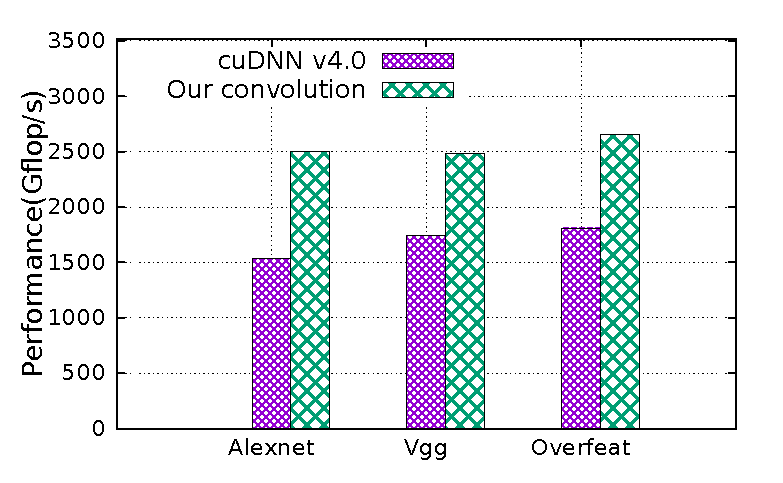
\includegraphics[scale=0.5]{cudnn}
\caption{cudnn vs convolution}
\label{fig:sgemm_tn}
\end{center}
\end{figure}
